% !TEX TS-program = pdflatex
% !TEX encoding = UTF-8 Unicode

% This is a simple template for a LaTeX document using the "article" class.
% See "book", "report", "letter" for other types of document.

\documentclass[11pt]{article} % use larger type; default would be 10pt


\usepackage[utf8]{inputenc} % set input encoding (not needed with XeLaTeX)

%%% Examples of Article customizations
% These packages are optional, depending whether you want the features they provide.
% See the LaTeX Companion or other references for full information.

%%% PAGE DIMENSIONS
\usepackage{geometry} % to change the page dimensions
\geometry{a4paper} % or letterpaper (US) or a5paper or....
% \geometry{margin=2in} % for example, change the margins to 2 inches all round
% \geometry{landscape} % set up the page for landscape
%   read geometry.pdf for detailed page layout information

\usepackage{graphicx} % support the \includegraphics command and options

% \usepackage[parfill]{parskip} % Activate to begin paragraphs with an empty line rather than an indent

%%% PACKAGES
\usepackage{booktabs} % for much better looking tables
\usepackage{array} % for better arrays (eg matrices) in maths
\usepackage{paralist} % very flexible & customisable lists (eg. enumerate/itemize, etc.)
\usepackage{verbatim} % adds environment for commenting out blocks of text & for better verbatim
 % make it possible to include more than one captioned figure/table in a single float
% These packages are all incorporated in the memoir class to one degree or another...

\usepackage[export]{adjustbox}
\usepackage{graphicx}
\usepackage{amssymb}
\usepackage{hyperref}
\hypersetup{
    colorlinks=true,
    linkcolor=blue,
    filecolor=magenta,      
    urlcolor=cyan,
}
\usepackage{relsize}
\usepackage[utf8]{inputenc}
\usepackage[LGR]{fontenc}
\usepackage[T1]{fontenc}
\usepackage[greek,english]{babel}
\usepackage{alphabeta}
\usepackage{amsmath}
\usepackage{physics}
\usepackage{amsfonts}
\usepackage{nccmath}
\usepackage[overload]{empheq}
\usepackage{float}
\usepackage{caption}
\usepackage{subcaption}
\restylefloat{table}
\usepackage{afterpage}
\usepackage[nottoc,notlot,notlof]{tocbibind}
\addto\captionsenglish{\renewcommand{\figurename}{Εικόνα}}


\begin{document}

\begin{titlepage}
    \begin{center}
        \vspace*{1cm}
	
\includegraphics[width=0.2\textwidth]{plots/ntua_logo}\\    
	\vspace*{1cm}
        \Huge
        \textbf{Αναγνώριση Προτύπων}
            
        \vspace{0.5cm}
        \LARGE
        Εργασία 1η
            
        \vspace{1.5cm}
        
        \textbf{Μιχάλης Στεφανής}\\    
        \textbf{Βασίλης Μηναδάκης}
            
        \vfill
                        
        \vspace{0.8cm}
            
        
            
        \Large
        Σχολή Ηλεκτρολόγων Μηχανικών και Μηχανικών Υπολογιστών\\
        Εθνικό Μετσόβιο Πολυτεχνείο\\
        Αθήνα\\
        24/10/2021
            
    \end{center}
\end{titlepage}

Για την επίλυση όλων των ερωτημάτων έγινε η χρήση των βιβλιοθηών numpy, scikit-learn και matplotlib της python.\\
Το πρώτο στάδιο αφορά την εισαγωγή των train και test δεδομένων από μορφή αρχείου κειμένου (.txt) στον κώδικα της python. Αυτό επιτυγχάνεται με τη χρήση της συνάρτησης $np.genfromtxt()$. Έπειτα, ακολουθώντας τις οδηγίες της εκφώνησης δημιουργήθηκαν ρα εξής arrays δεδομένων:

\begin{table}[h]
\begin{center}
\begin{tabular}{c c }
\hline\hline
Ονομασία & Διαστάσεις \\
\hline
train\_features & 7291x256\\ 
train\_labels     & 7291      \\  
test\_features  & 2007x256\\
test\_labels      & 2007\\
\hline 
\end{tabular}
\caption{Διαστάσεις των training και test dataset.}
\end{center}
\end{table}

Στο 2ο βήμα σχεδιάστηκε το υπ'αριθμόν 131 ψηφίο των train δεδομένων χρησιμοποιώντας συναρτήσεις της βιβλιοθήκης matplotlib και συγκεκριμένα της $plt.imshow()$ και $plt.show()$. Η πρώτη εφαρμόζεται ουσιαστικά πάνω στο 131ο στοιχείο των train\_features και η εικόνα που παράγεται είναι η κάτωθι.

\begin{figure}[H]
    \centering
    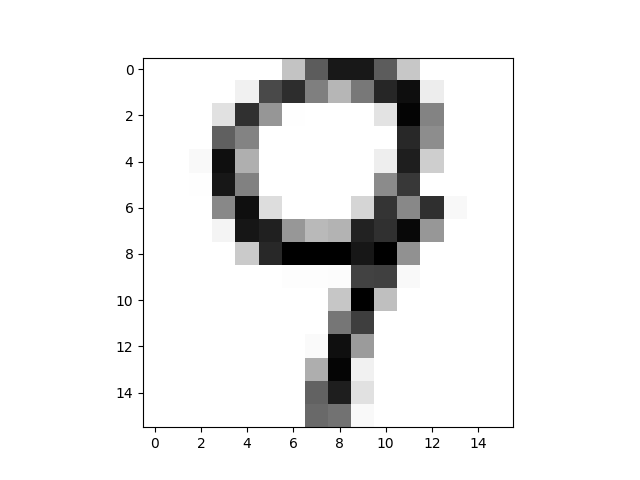
\includegraphics[width=0.7\textwidth]{plots/Step 2}
    \caption{Απεικόνιση του 131ου ψηφίου των train\_features.}
    \label{fig:step_2}
\end{figure}

Για το επόμενο βήμα (Βήμα 3) δομήθηκε η συνάρτηση $plot\_digits\_samples(X, y)$, της οποίας τα ορίσματα είναι τα training\_features και τα training\_labels αντίστοιχα. Συνοπτικά, η συγκεκριμένη συνάρτηση λειτουργεί με μία επαναληπτική διαδικασία από το 1 έως το πλήθος των στοιχείων του X (train\_features), εντός της οποίας αν το στοιχείο y(i) υπάρχει στο διάνυσμα $digits = \{0,1,...,9\}$, τότε σχεδιάζεται το αντίστοιχο ψηφίο και στη συνέχεια αφαιρείται από το διάνυσμα digits, μέχρι να μην υπάρχει κανένα στοιχείο πλέον εντός του digits. Η ενσωμάτωση των εικόνων και των 10 διαφορετικών ψηφίων σε μία εικόνα γίνεται με τη χρήση της συνάρτησης $plt.subplots()$ και παρουσιάζονται στην εικόνα \ref{fig:step_3}.

\begin{figure}[H]
    \centering
    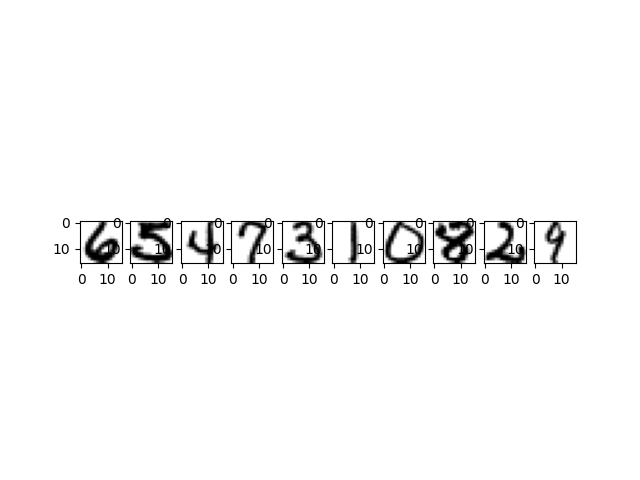
\includegraphics[width=1.1\textwidth]{plots/Step 3}
    \caption{Απεικόνιση του 131ου ψηφίου των train\_features.}
    \label{fig:step_3}
\end{figure}

Στη συνέχεια, για την υλοποίηση του 4ου βήματος, κατασκευάστηκε η συνάρτηση $mean\_value\_at\_pixel\_of\_digit(X, y, digit, pixel=(10, 10))$, η οποία υπολογίζει τη μέση τιμή όλων των χαρακτηριστικών ενός συγκεκριμένου pixel (συγκεκριμένα του 10ου) για το training set και δέχεται σαν input  τα train\_features, τα train\_labels και το ψηφίο που μας ενδιαφέρει (στη συγκεκριμένη περίπτωση το 0). Ο τύπος τις μέσης τιμής που χρησιμοποιήθηκε είναι η \ref{mean_value}: 

\begin{equation}
\label{mean_value}
\mu = \frac{1}{n}\bigg(\sum_{i=1}^{n}x_{i}\bigg),
\end{equation}
όπου $n$ το πλήθος των χαρακτηριστικών του pixel (10,10) για το ψηφίο 0.
\\

Στο βήμα 5 η λογική που ακολουθήθηκε είναι όμοια με αυτή του προηγούμενου βήματος, μόνο που σε αυτή την περίπτωση το function που δομήθηκε ($mean\_value\_at\_pixel\_of\_digit(X, y, digit, pixel=(10, 10))$) κάνει τους υπολογισμούς με βάση της διασπορά των χαρακτηριστικών, δηλαδή γίνεται χρήση της σχέσης \ref{variance}: 

\begin{equation}
\label{variance}
Var(x) = \frac{1}{n}\bigg(\sum_{i=1}^{n}(x_{i}-\mu)^{2}\bigg).
\end{equation}
Εφαρμόζοντας τις δύο παραπάνω συναρτήσεις για το 10 pixel όλων των χαρακτηριστικών του ψηφίου μηδέν προκύπτουν οι εξής τιμές για τη μέση τιμή και διασπορά του:

\begin{table}[h]
\begin{center}
\begin{tabular}{c c c}
\hline\hline
 & Μέση Τιμή & Διασπορά\\
\hline
10ο pixel του 0 & -0.0826 & 0.115\\
\hline 
\end{tabular}
\caption{Αποτελέσματα μέσης τιμής και διασποράς του 10ου pixel όλων των στοιχείων για το ψηφίο 0.}
\end{center}
\end{table}

Στη συνέχεια (Βήμα 6) για τον υπολογισμό της μέσης τιμής και της διασποράς των χαρακτηριστικών όλων των pixel ενός οποιουδήποτε ψηφίου, δομήθηκαν οι συναρτήσεις $digit\_mean(X, y, digit)$ και $digit\_variance(X, y, digit)$. Αυτές οι δύο συναρτήσεις σε πρώτο επίπεδο υπολογίζουν τη μέση τιμή και τη διασπορά κάθε ενός pixel του επιθμητού ψηφίου και στη επιστρέφει αυτές τις τιμές σε ένα διάνυσμα. 

Οι τελευταίες δύο συναρτήσεις χρησιμοποιούνται ως εσωτερικές της νέας συνάρτησης $plot\_digit\_mean(X, y, digit)$, η οποία χρησιμοποιείται για το σχεδιασμό ενός επιθμητού ψηφίου χρησιμοποιώντας τη μέση τιμή όλων των pixel όλων των χαρακτηριστικών του συγκεκριμένου ψηφίου. Η εικόνα που παράγεται με τη χρήση του συγκεκριμένου function για το ψηφίο 0, χρησιμοποιώντας το training set είναι η εικόνα \ref{fig:step_7}.

\begin{figure}[H]
    \centering
    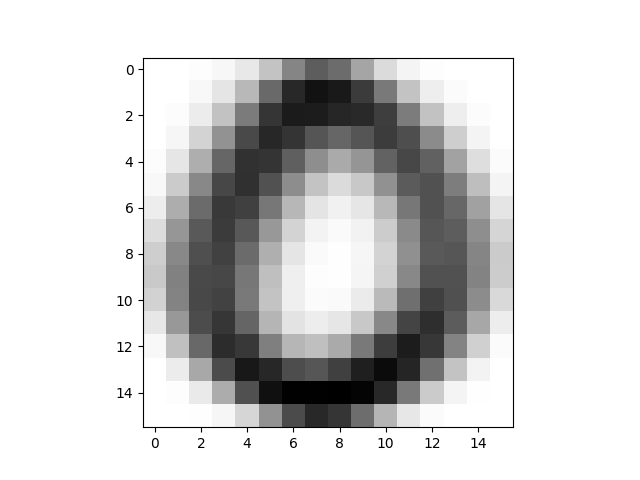
\includegraphics[width=0.7\textwidth]{plots/Step 7}
    \caption{Απεικόνιση του ψηφίου 0 με τη χρήση της μέσης τιμής των pixel όλων των χαρακτηριστικών του training set.}
    \label{fig:step_7}
\end{figure}

Το επόμενο βήμα (\textbf{Βήμα 8}) είναι να σχεδιάσουμε ένα από τα ψηφία που επιθυμούμε χρησιμοποιώντας όχι την μέση τιμή, αλλά την διασπορά των pixel των είκονων που αντιπροσωπεύουν το επιθυμητό ψηφίο. Αυτό γίνεται με την συνάρτηση $plot\_digit\_variance$. Για παράδειγμα, για το ψηφίο $0$ παίρνουμε την εξής εικόνα:

\begin{figure}[H]
    \centering
    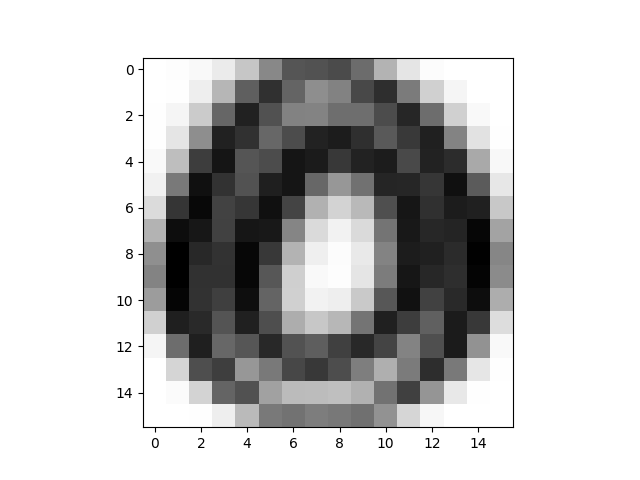
\includegraphics[width=0.7\textwidth]{plots/variance_0}
    \caption{Απεικόνιση του ψηφίου $0$ μέσω της διασποράς των pixel}
    \label{fig:var_0}
\end{figure}



Αν συγκρίνουμε την εικόνα που πήραμε από το ψηφίο 0 μέσω της μέσης τιμής με αυτήν που πήραμε μέσω τις διασποράς θα παρατηρήσουμε κάποιες σχετικά αναμενόμενες διαφορές. Η εικόνα που αντιστοιχεί στην διασπορά έχει τα πιο σκούρα της pixels αυτά που τα αντίστοιχα στην εικόνα της μέσης τιμής είναι τα λιγότερο σκούρα. Για παράδειγμα τα pixels της εικόνας της μέσης τιμής για το $0$ είναι περισσότερο σκούρα στις δύο "κορυφές" του $0$. Αντίστοιχα, τα pixels της εικόνας της διασποράς είναι λιγότερο σκούρα (περισσότερο γκρί παρά μαύρα) στις κορυφές αυτές. Αυτό είναι αναμενόμενο, καθώς η διασπορά είναι στην ουσία η απόσταση μιας μεταβλητής από την μέση τιμή της. \\

Για το \textbf{Βήμα 9} υπολογίζουμε την μέση τιμή και την διασπορά όλων των pixel για όλα τα δεδομένα εκπαίδευσης. Αυτό μπορεί να γίνει πολύ απλά χρησιμοποιωντας list-comprehension της python και τις συναρτήσεις $digit\_mean$ και $digit\_variance$ αντίστοιχα. Παίρνουμε έτσι δύο λίστες 10 γραμμών και 256 στηλών ($mean\_X$ και $var\_X$). Κάθε γραμμή αντιστοιχεί σε ένα ψηφίο και κάθε στήλη στην μέση τιμή και την διασπορά του εκάστοτε pixel. \\

Για να σχεδιάσουμε όλα τα ψηφία χρησιμοπoιούμε τις συνάρτησεις  $plot\_digits\_by\_mean$ και $plot\_digits\_by\_variance$, οι οποίες χρησιμοποιούν 10 φορές η καθε μία τις συναρτήσεις $digit\_mean$ και $digit\_variance$ αντίστοιχα. 

\begin{figure}[H]
    \centering
    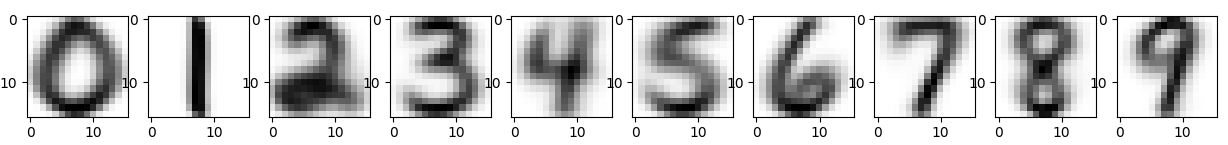
\includegraphics[width=1.1\textwidth]{plots/all_digits_mean}
    \caption{Απεικόνιση όλων των ψηφίων μέσω της μέσης τιμής των pixel}
    \label{fig:all_mean}
\end{figure}

\begin{figure}[H]
    \centering
    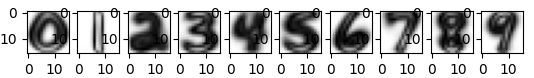
\includegraphics[width=1.1\textwidth]{plots/all_digits_variance}
    \caption{Απεικόνιση όλων των ψηφίων μέσω της διασποράς των pixel}
    \label{fig:all_mean}
\end{figure}


Από το \textbf{Βήμα 10} και μετά ξεκινούν οι δοκιμές του ταξινομητή της Ευκλείδιας απόστασης. Αυτός υλοποιείται με την βοήθεια δύο συναρτήσεων. Η συνάρτηση $euclidean\_distance$ υπολογίζει την Ευκλείδια απόσταση μεταξύ δύο διανυσμάτων (ή πινάκων) μέσω της σχέσης:

\begin{equation}
\displaystyle d(A, B) = \sqrt{(A[1] -B[1]) ^ 2 + (A[2] - B[2]) ^ 2 + \dots + (A[N] - B[N]) ^ 2}
\end{equation}

Στην συνέχεια για την ταξινόμηση των στοιχείων του test set καλούμε την συνάρτηση $euclidean\_distance\_classifier$. Η συνάρτηση αυτή παίρνει ως ορίσματα τα χαρακτηριστικά του test set (test features) καθώς και την λίστα που περιλαμβάνει τις μέσες τιμές όλων των ψηφίων του training set. Υπολογίζει για το κάθε στοιχείο του test set τις ευκλείδιες αποστάσεις του στοιχείου αυτού από τις μέσες τιμές. Επιλέγεται η μικρότερη από αυτές, η οποία ελάχιστη απόσταση είναι αντιπροσωπευτική της κλάσης στην οποία ταξινομήθηκε τελικά το στοιχείο που επιλεξαμε.\\

Ως πρώτη δοκιμή του ταξινομητή, διαλέγουμε το στοιχείο υπ'αριθμόν 101 των test δεδομένων και το δίνουμε ως είσοδο στον ταξινομητή μας. Για να έχουμε μία καλύτερη εικόνα, το στοιχείο αυτό είναι το εξής:


\begin{figure}[H]
    \centering
    \includegraphics[width=0.7\textwidth]{plots/figure_101}
    \caption{Το ψηφίο υπ'αριθμόν 101 των test δεδομένων}
    \label{fig:101}
\end{figure}

Αν τρέξουμε τον ταξινομητή μας θα διαπιστώσουμε ότι η ταξινόμηση δεν είναι σωστή. Όπως μπορούμε να διακρίνουμε στην παραπάνω εικόνα, το ψηφίο που αναπαριστά είναι το $6$. Παρόλα αυτά ο ταξινομητής δίνει την πρόβλεψη $0$. Οπότε "μπερδεύει"το παραπάνω εξάρι με μηδενικό. Αυτό δεν πρέπει να μας αποθαρρύνει αφού ένα μόνο test δεδομένο δεν αρκεί για να βγάλουμε συμπέρασμα για τον ταξινομητή μας. Εξάλλου η παραπάνω εικόνα είναι πράγματι ένα ασυνήθιστο $6$ για τα τυπικά χειρόγραφα δεδομένα.\\

Ερχόμαστε τώρα στο \textbf{Βήμα 11}, όπου τροφοδοτούμε τον ταξινομητή μας με όλα τα test δεδομένα. Η συνάρτηση $euclidean\_distance\_classifier$ θα μας γυρίσει ένα \% ποσοστό επιτυχίας (δηλαδή τον αριθμό των δεδομένων που ταξινομήθηκαν επιτυχώς διαιρεμένο με τον συνολικό αριθμό των δεδομένων) και μία λίστα με όλες τις προβλέψεις του ταξινομητή (δηλαδή μία λίστα που θα μας λέει σε ποια κατηγορία ταξινομήθηκε το κάθε test δεδομένο). Αν τρέξουμε τον κώδικα και τυπώσουμε τις τιμές τότε θα λάβουμε στην οθόνη μας:

\begin{center}
The accuracy of the euclidean distance classifier is: 81.42 \%
\end{center}

To ποσοστό αυτό είναι αρκετά ικανοποιητικό για τον περιορισμένο αυτό όγκο δεδομένων που είχαμε στην διάθεσή μας.\\


Στο \textbf{Βήμα 12} υλοποιούμε τον ταξινομητή της Ευκλείδιας απόστασης σαν έναν scikit-learn estimator. Ουσιαστικά δημιουργούμε μία κλάση EuclideanDistanceClassifier της python, μέσα στην οποία θα καλούμε τις κατάλληλες συναρτήσεις που έχουμε ήδη σχηματίσει προηγουμένως στον κώδικα. Η μόνη μεταβλητή που θα αρχικοποιείται στην κλάση είναι η μέση τιμή των κατηγοριών (των ψηφίων) και αυτή θα υπολογίζεται στην συνέχεια από την συνάρτηση fit μέσω των train δεδομένων. Η συνάρτηση predict θα έχει ως είσοδο τα test features και θα επιστρέφει την λίστα με τις προβλέψεις του ταξινομητή, ενώ η συνάρτηση score θα έχει ως είσοδο τα test features και τα test labels επιστρέφει το ποσοστό επιτυχίας.\\

Αν θέλουμε να καλέσουμε τώρα τον ταξινομητή μας σαν να ήταν ταξινομητής του scikit-learn θα πρέπει απλά να καλέσουμε την κλάση μας ώς:
\begin{center}
clf  = EuclideanDistanceClassifier()
\end{center}

Στην συνέχεια θα πρέπει να τροφοδοτήσουμε τα train δεδομένα στην κλάση για να υπολογίσουμε τις μέσες τιμές, μέσω της συνάρτησεις fit:
\begin{center}
clf.fit(out training features)
\end{center}

Τέλος, αν θέλουμε να μας επιστραφούν οι προβλέψεις ή η ακρίβεια του ταξινομητή καλούμε τις συναρτήσεις predict ή score αντίστοιχα:
\begin{center}
clf.predict(our test features)\\
clf.score(our test features, our test labels)
\end{center}

Προφανώς αν τυπώσουμε το score μέσω της παραπάνω κλάσης θα λάβουμε το ίδιο ακριβώς αποτέλεσμα με την συνάρτηση $euclidean\_distance\_classifier$.\\

Στο \textbf{Βήμα 13} εξερευνούμε λίγο παραπάνω τον ταξινομητή που δημιουργήσαμε υπολογίζοντας το cross-validation-score με την χρήση της τεχνικής K-Folding καθώς επίσης σχεδιάζουμε την περιοχή απόφασης και την καμπύλη εκμάθησης του ταξινομητή.\\

Για τον υπολογισμό του cross-validation-score αντλούμε από το scikit-learn τις κλάσεις ΚFOLD και $cross\_val\_score$. Στην συνέχεια καλούμε την συνάρτηση $k\_fold\_cv$ η οποία παίρνει ως είσοδο τα train features και τα train labels και τυπώνει το cross-validation-score και το cross-validation-error. Αναμένουμε σαν cross-validation-score να λάβουμε κάτι λίγο παραπάνω από το score του ταξινομητή μας. Πράγματι, αν καλέσουμε την συνάρτηση τότε θα λάβουμε στην οθόνη:
\begin{center}
The 5-fold cross-validation score is 84.858036 +-0.181618\\
The 5-fold cross-validation error is 15.141964 +-0.181618
\end{center}

Το ποσοστό του cross-validation είναι περίπου 85 \%, λίγο μεγαλύτερο από το 82 \% του ταξινομητή.



Τέλος σχεδιάζουμε την καμπύλη εκμάθησης του ταξινομητή μας. Αυτό γίνεται μέσω της συνάρτησης $plot\_learning\_curve$. Παίρνει ως είσοδο τον ταξινομητή (την κλάση που τον αντιπροσωπεύει) και όλα τα train δεδομένα (features, labels). 

\begin{figure}[H]
    \centering
    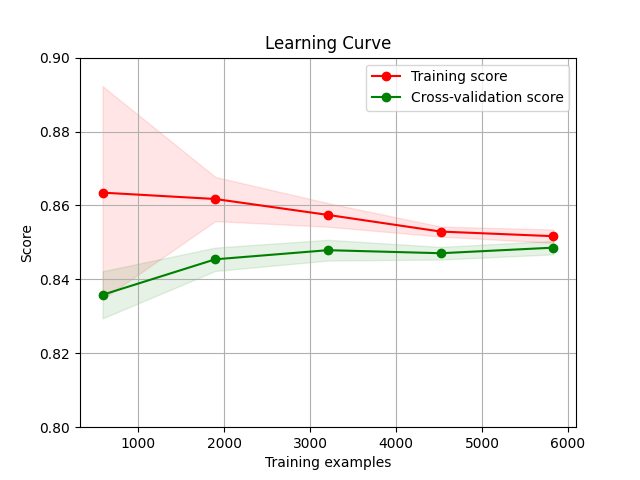
\includegraphics[width=0.7\textwidth]{plots/learning_curve.png}
    \caption{Η καμπύλη εκμάθησης του Ευκλείδιου ταξινομητή}
    \label{fig:learningcurve}
\end{figure}

Όπως αναμέναμε, το cross-validation-score αρχικά αυξάνεται και, όσο προχωρά η εκπαίδευση, τείνει να εξισωθεί με το training score.

 
\end{document}